% NIH Grant Proposal for the Specific Aims and Research Plan Sections
%----------------------------------------------------------------------------------------
%	PACKAGES AND OTHER DOCUMENT CONFIGURATIONS
%----------------------------------------------------------------------------------------

\documentclass[11pt,notitlepage]{article}

% A note on fonts: As of 2013, NIH allows Georgia, Arial, Helvetica, and Palatino Linotype. LaTeX doesn't have Georgia or Arial built in; you can try to come up with your own solution if you wish to use those fonts. Here, Palatino & Helvetica are available, leave the font you want to use uncommented while commenting out the other one.

\usepackage[super]{natbib}
\usepackage{palatino} % Palatino font
%\usepackage{helvet} % Helvetica font
\renewcommand*\familydefault{\sfdefault} % Use the sans serif version of the font
\usepackage[T1]{fontenc}
\linespread{1.05} % A little extra line spread is better for the Palatino font
\usepackage{hyperref} % to allow hyperlinks to websites on the internet
\usepackage[hypcap]{caption} % to point to the top of the image
\usepackage{lipsum} % Used for inserting dummy 'Lorem ipsum' text into the template
\usepackage{amsfonts, amsmath, amsthm, amssymb} % For math fonts, symbols and environments
\usepackage{graphicx} % Required for including images
\usepackage{booktabs} % Top and bottom rules for tables
\usepackage{wrapfig} % Allows in-line images
%\usepackage[labelfont=\small]{caption} % Make figure numbering in captions bold
\usepackage[top=0.6in,bottom=0.6in,left=0.6in,right=0.6in]{geometry} % Reduce the size of the margin

\usepackage{booktabs}
\usepackage{graphicx}
\usepackage[table,xcdraw]{xcolor}
\pagestyle{empty} % Remove page numbers
%\let\oldtabular\tabular 
%\renewcommand{\tabular}{\large\oldtabular}

\hyphenation{ionto-pho-re-tic iso-tro-pic fortran} % Specifies custom hyphenation points for words or words that shouldn't be hyphenated at all

  % to reduce white space between SECTIONS
\usepackage[compact]{titlesec}
\titlespacing{\part}{0pt}{*0pt}{*0pt}
\titlespacing{\section}{0pt}{*0}{*0}
\titlespacing{\subsection}{0pt}{*0}{*0}
\titlespacing{\subsubsection}{0pt}{*0}{*0}

% Reduce whitespace arount lists
\usepackage{mdwlist}
\usepackage{verbatim}
%\usepackage[compact]{titlesec}
%\titlespacing{\part}{-200pt}{-100pt}{-200pt}
%\titlespacing{\section}{0pt}{0pt}{0pt}
%\titlespacing{\subsection}{0pt}{*0}{*0}
%\titlespacing{\subsubsection}{-2pt}{*0}{*0}
%\titlespacing{\subparagraph}{-5pt}{*0}{*0}
%\titlespacing*{\subparagraph} {\parindent}{1ex plus 1ex minus .2ex}{0.5em}

  
  % to reduce white space between PARAGRAPHS
%\setlength{\parskip}{-2pt}
% \setlength{\parsep}{-2pt}

  % additional parameters
\setlength{\headsep}{20pt}
%\setlength{\topskip}{0pt}
%\setlength{\topmargin}{0pt}
%\setlength{\topsep}{0pt}
\setlength{\partopsep}{-2pt}
%\setlength{\parindent}{1cm}

% to reduce white space around figures
% \setlength{\textfloatsep}{0pt plus 0pt minus 0pt}

% Set graphics path to tell latex where to look for images
%\graphicspath{ {C:/Users/Micheal/Dropbox/Professional/KL2/BigDataR01/ConceptGraphics/} }

\begin{document}
\section*{Specific Aims}
National health databases and electronic health records (EHR) are inherently incomplete but
clustered by procedure, provider, service, institution and geography. Often 
neglected, this rich spatial and temporal organization is most realistically 
captured in hierarchical statistical models with cluster-specific parameters, but 
estimating such models is still difficult for medical researchers using traditional software,
particularly when data on some units of observation are uncollected or otherwise missing.
We propose to further develop the capabilities of the software called \textit{Stan} --- 
which is a probabilistic programming language, mathematical library, suite of estimation
algorithms, and ecosystem of supporting interfaces --- in order to make advanced hierarchical  
modeling accessible to data scientists doing medical outcomes research with incomplete data.
\textit{Stan} has the potential to transform the way medical outcomes research is conducted.

\paragraph*{Flexibility and robustness of hierarchical modeling could 
transform EHR based outcomes research.} Consider surgery as an 
illustrative example. Patients in the same hospital undergoing the 
same surgical intervention by the same team will show similar clinical 
trajectories and responses. We are interested in investigating
differences in therapeutic effects or to predict adverse outcomes in order to prevent 
them. Doing so entails (1) estimating individual intercept-shifts for each provider and procedure
can help to control for potentially confounding differences 
in quality of care by different teams, (2) allowing for spatial clustering of adherence 
behavior, e.g., by different services, which can be represented by multilevel modeling, and
(3) partially pooling estimates to improve precision, especially in subgroups with sparse data.
Prediction of adverse health outcomes can be improved by exploiting the implied correlations between different but related subsets of data. 
Conversely, failure to account for the highly structured and correlated nature of health care delivery or
failure to account for the mechanisms by which some data are missing may lead 
to incorrect statistical inferences, poor predictions, and adverse health consequences. 
Realistic modeling of the heterogeneity in  care delivered may help to identify reasons for differences in outcomes.
All of these features can be incorporated into a model specified using the Stan language.

\paragraph*{Classical approaches and traditional software often lack flexibility 
for hierarchical modeling.} Most available software limits the types of 
hierarchical models that can be estimated because their algorithms are more likely 
to run into computational problems when estimating more complicated hierarchical models.
In contrast, \textit{Stan} is a flexible, general-purpose modeling language and a 
novel, powerful estimation engine that has facilitated 
advanced hierarchical modeling in biostatistics, epidemiology, public health, 
political science, and pharmacokinetics. \textit{Stan's} development has been funded 
by the NSF, DoD, and other organizations. \textit{Stan} and the interfaces to it
(e.g. from \textit{Python, Julia, R}, etc.) are open source and platform-independent.

\paragraph*{Good hierarchical modeling requires good model diagnostics} 
We lack intuitive visual and exploratory diagnostic tools to recognize when a complicated model is logically 
flawed or fails to fit the data empirically. We propose to further enhance \textit{Stan} and its ecosystem of 
\textit{Stan}-related software to incorporate interactive and intuitive statistical tools to facilitate principled model 
checking and respecification.

\paragraph*{Aim 1:} To further develop the most user-friendly interface to \textit{Stan}, 
which is a package called \textit{rstanarm} for the open-source statistical language and 
environment \textit{R}, in order to make it more suitable for clinical data 
scientists and biostatisticians that want to estimate hierarchical models for EHR data.

\paragraph*{Aim 2:} To further develop \textit{shinystan}, our interactive web application to 
analyze and visually explore the output of \textit{Stan} models and to develop diagnostics 
to identify and troubleshoot computational and empirical problems with advanced hierarchical models.

\paragraph*{Aim 3:} To further develop \textit{mi}, our \textit{R} package for multiple imputation
of missing data so that it can make use of \textit{Stan} via the models provided by \textit{rstanarm}.

\paragraph*{Aim 4:} To explicate, document, and disseminate realistic hierarchical 
models for incomplete data to the clinical data science community with hands on use cases, workshops, journal articles, and 
online tutorials. To solicit the data scientist community feedback, engage new 
software developers, and to incorporate improvements to our software.

\section*{Research Strategy}

\section*{Significance}

\section*{The nested structure of health care delivery and electronic health data}
Clinical data scientists are faced with an abundance of useful electronic health data, 
but limitations of traditional estimators constrain the scientific hypotheses they can explore. 
Electronic health related data sets are growing rapidly in the number of units of observation and 
variables observed. This growth implies that we can investigate increasingly fine-grained 
models. Whereas before we were limited to models of the mean structure and effect, we 
now want to our models to account for clinical heterogeneity.

\subparagraph*{The National Anesthesia Clinical Outcomes Registry (NACOR)} illustrates 
the clustered, nested data structure of contemporary health  care delivery and electronic health data capture. 
NACOR is maintained by the Anesthesia Quality Institute and funded by the American Society of 
Anesthesiologists. We will utilize NACOR as a use case for dissemination in workshops for perioperative data scientists.

\subparagraph*{Perioperative health care delivery and data capture are nested and clustered.}
Anesthesia is an illustrative case of the how health care is increasingly 
electronically documented, which facilitates the continuous collection of 
physiological data and therapeutic interventions during critical periods. 
This electronically captured data 
is joined with surgical and anesthesia procedure codes, International 
Classification of Disease codes, provider identifiers, patient perioperative 
risk, outcome and provider compliance assessment. Participating institutions upload 
this comprehensive file from their anesthesia information management systems
directly to NACOR. NACOR contains at present over 30 million individual 
electronic records of anesthesia care provided and, like similar databases, is 
growing rapidly. This data set invites health services and outcomes research, 
but (see letter of support by Dr. Dutton, last director or 
NACOR and Dr. Kheterpal director of MPOG, the other large perioperative EHR 
database) their exploitation is limited by the lack of accessible software to investigate 
important scientific questions with realistic hierarchical models.

\subparagraph*{Outcomes and care delivered depend on procedure, provider, and patient characteristics.} 
We explain the hierarchical structure of health care delivery with our NACOR model on anesthesia quality \cite{AndreaeWhite2015}. 
The (dichotomous) outcome (e.g., postoperative nausea) of 
an anesthetic for a given individual will depend on the surgical procedure the patient is undergoing and under 
which service, but also on the local institutional culture and indeed the individual anesthesia provider and 
his or her qualifications and preferences (Figure \ref{fig:NACOR}).

\begin{wrapfigure}{l}{0.4\textwidth} 
\vspace*{-12pt}
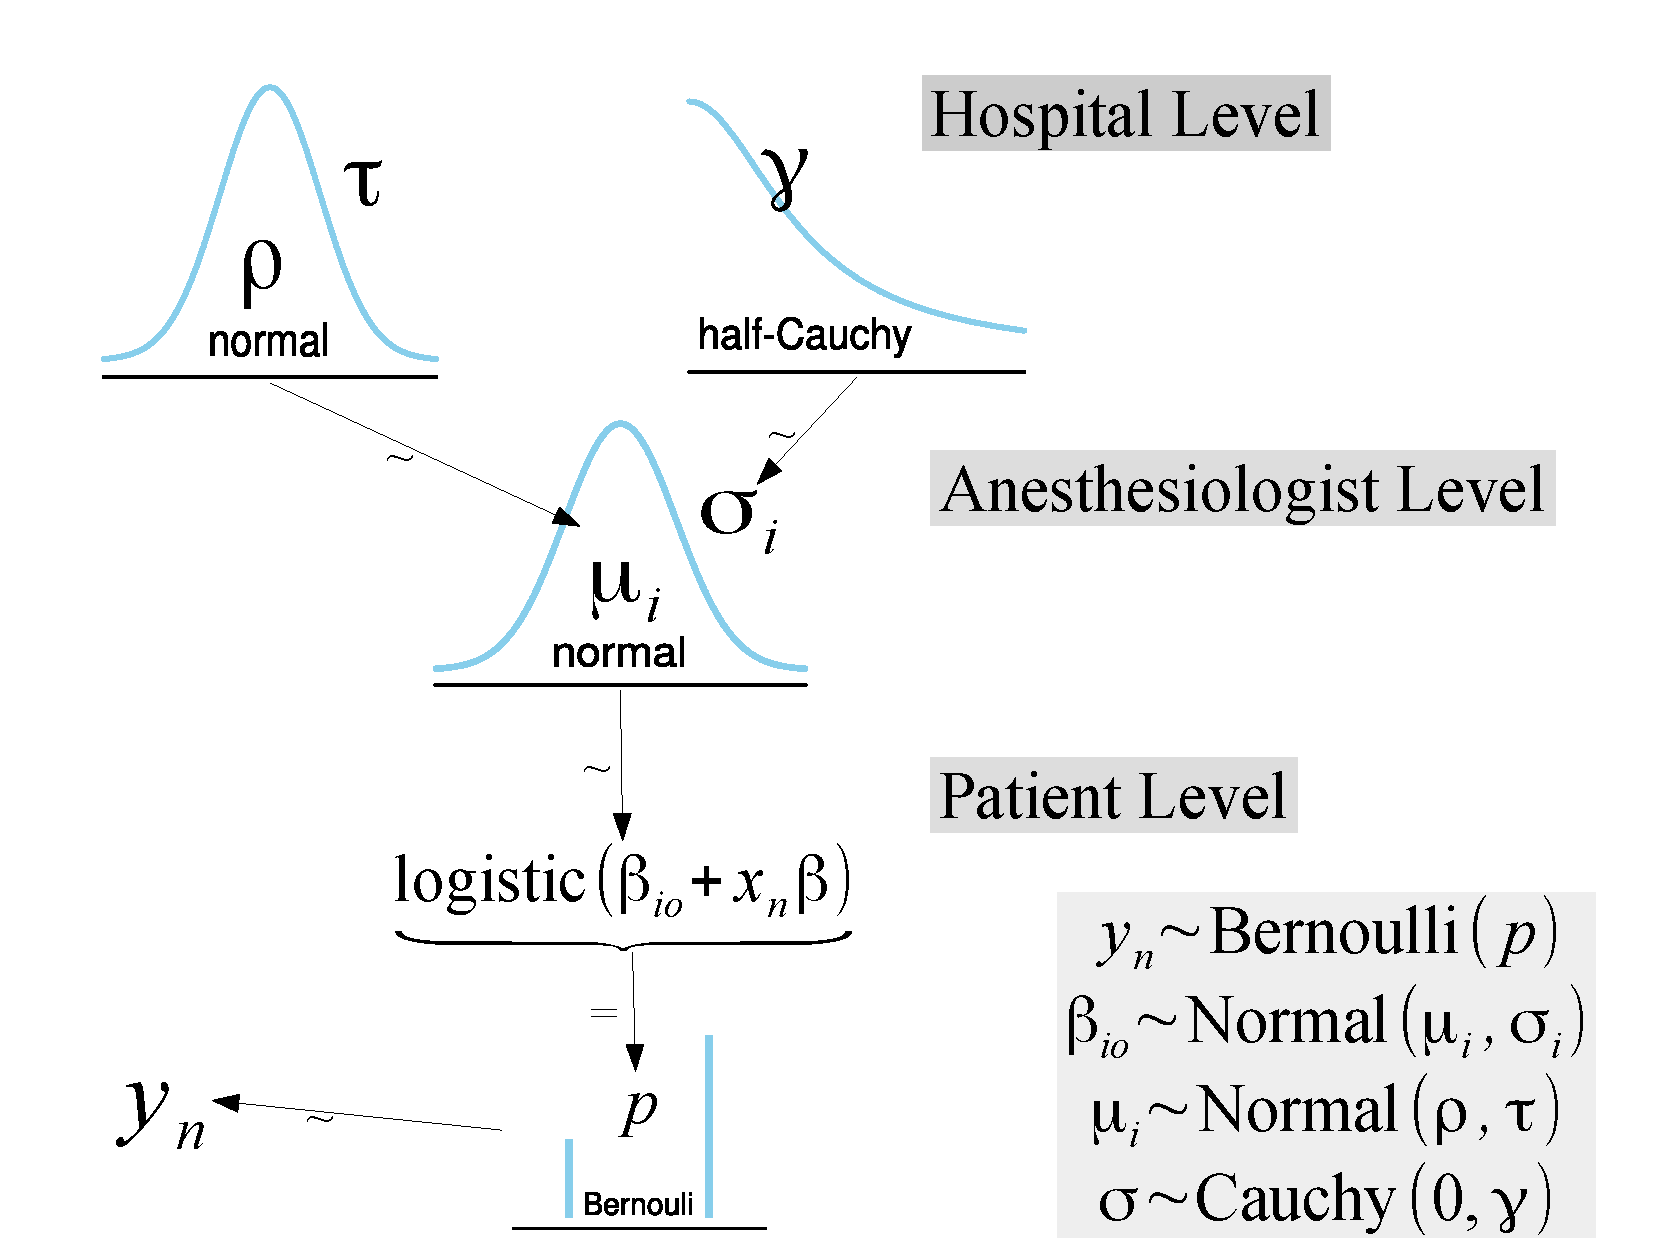
\includegraphics[width=0.4\textwidth]{Figures/DistrogramNACOR.pdf} 
\caption{Hierarchical structure of health care delivered in the perioperative setting.}
\label{fig:NACOR}
\vspace*{-12pt}
\end{wrapfigure} 

Outcome $y_n$ for the $n$th patient is a Boolean indicator to be predicted by a logistic regression. We allow the patient-specific
intercept $\beta_{oi}$ to vary according to the $i$th anesthesiology provider caring for the patient. The provider level mean 
$\mu_i$ and within-provider variance $\sigma_i$ vary by hospital. $x_n$ is a vector of patient level predictors, and $\beta$ is a vector 
of regression coefficients.  

Two more examples illustrate the nested structure of health care outcomes: 
Anesthesiologists may feel more or less inclined or competent to offer 
regional anesthesia for labor pain. Provision of epidural labor 
anesthesia varies widely across the nation and within an institution and 
is predicted by socioeconomic and racial patient characteristics 
\cite{Rust2004,Glance2007}.  
While an average a neurosurgeon may have less blood loss during spine 
surgery, a particularly gifted orthopedic surgeon may outperform the 
average neurosurgeon with regards to blood loss.

\section*{Hierarchical models capture contemporary health care practice realistically}
Hierarchical modeling could transform electronic health records based 
outcomes research, because the rich spatial and temporal 
organization of electronic health records is most realistically 
captured in hierarchical statistical models. However, the estimation of such models
is still difficult, both statistically and computationally.  
Additional depth of data (simply adding units of observation) will increase 
the precision of estimates and generally make our clinical data analysis easier. 
However, there is also more breadth to the data: 
more subgroups, locations, provider or time granularity than is currently 
being modeled. Incomplete and noisy measurements cannot easily be incorporated into standard models.
Individual patient data do not easily fit traditional meta-analysis
\cite{Andreae2015,Andreae2012}.

\subsection*{Modeling the multifaceted correlations in EHR is reflecting actual clinical practice}
To realistically model the multifaceted correlations seen in actual clinical 
practice, we specified a logistic regression model  (Figure~ \ref{fig:NACOR}) 
that predicts anesthesia quality in the NACOR database
with regression coefficients that vary by provider, where providers 
are again nested by service or by hospital 
\cite{AndreaeWhite2015}. We also need to adjust for the type of surgical procedure, and there are 
thousands of different surgical procedures performed in the NACOR data. The number 
of parameters to estimate grows very quickly and so do the potential interactions. This so-called
incidental parameters problem violates the assumptions that are necessary for maximum likelihood
estimators to be consistent, even if the dataset has a very large number of observations.
One solution lies in hierarchical modeling, where we estimate hyper-parameters and allow
lower-level parameters to vary across groups \cite{Bafumi_Gelman_2007}. 
In hierarchical models, we can borrow strength from larger groups and thereby improve estimates for 
smaller subgroups \cite{ParkGelman2004bayesian}.

\subsection*{Hierarchical models provide efficient inferences with partial pooling}
Inference based on partial pooling outperforms (a) the no-pooling and (b) the 
complete-pooling approaches, as can be shown mathematically \cite{Efron_1975} 
or via cross-validation \cite{Gelman-Hill_2014}: In frequentist terminology, by trading an increase in 
bias for a reduction in variance, hierarchical modeling can reducing the mean square error both
in estimating unknowns and in predicting future outcomes.

(a) The no-pooling approach entails estimate the model separately for each mutually exclusive and
exhaustive subsets of the data. Howerver, despite the richness of the EHR data, there are far too many 
sub-classifications (e.g., one model for each type of surgery) to make useful inferences.

(b) Complete pooling constitutes the other extreme of the spectrum, but the equality constraints 
imposed on the coefficients across all subgroups may be violated by the data-generating process. 
Ignoring obvious differences in the way the data are generated --- such 
as between patients undergoing tracheotomy versus cesarean section --- glosses
over the granular detail that is readily available in EHR data.

We choose the middle ground: inference using partial pooling or hierarchical modeling is especially effective 
for our richly organized NACOR data set because the estimate of each individual parameter is informed by data from 
all the other patients in our cohort, which improves prediction especially for subgroups with sparse data. \cite{Gelman2009} 
Efron explained this apparent paradox well to non-statisticians in the 
\href{http://www.nature.com/scientificamerican/journal/v236/n5/pdf/
scientificamerican0577-119.pdf}{Scientific American}
\cite{Stein_paradox_Scientific_American}. 
Our co-investigator, Dr. Hall, recently applied this approach to seizure prediction \cite{Hall2009a}.

\subsubsection*{Borrowing strength is beneficial even in very large data sets}
In summary, the geographic, spatial and other heterogeneities outlined above  
can undermine the precision of estimates or predictions even for 
extremely large clinical data sets. Partial pooling can improve estimation and prediction
by borrowing strength from different but related groups
\cite{Tukey1963borrowing,Jones1986collected}. 

\section*{Meta-analysis: hierarchical modeling of outcomes research}
Systematic reviews and meta-analysis \cite{Sackett1996} --- the synthesis of trial data 
to support clinical decision making --- is another example of hierarchical modeling where traditional software and 
classical modeling approaches limit progress in data-intensive outcomes research \cite{Andreae2015}.  
Evidence synthesis (a more accurate term than meta-analysis) is a powerful tool 
to pool clinical trials and provide the highest level guidance for clinical care\cite{Ashby2000,Cook1997}. 

\subsection*{Variance in study design and outcome reporting hamper evidence synthesis}
However, studies on perioperative outcomes tend to vary in design and reported outcomes\cite{Andreae2013}, making 
evidence synthesis challenging with classical frequentist statistical models \cite{Spiegelhalter_11134920}, (see 
letter of support by Dr. Sacks). Different study designs can make it difficult to perform meta-analysis or meta-regression 
with classical methods and standard systematic review software \cite{Deeks2011chapter}. Classical meta-analysis may also 
underestimate the between-study-variability for small numbers of trials \cite{Song2012,Cornell2014,Andreae2015}. 
Classical meta-analysis is an example of data with a \textit{single} level of hierarchical grouping: patients' 
outcomes are grouped within clinical trials \cite{egger2008systematic}. There are however several constraints and limitations 
with this classical approach to meta-analysis that could be overcome with more sophisticated hierarchical modeling  
\cite{Andreae2015,Thompson2002,Abroug2011}.

\subsubsection*{Hierarchical models integrate all available data for evidence synthesis}

Trial or population characteristics may introduce another level of grouping, for example pooling long-term outcomes 
after regional anesthesia by surgical intervention \cite{Andreae2013,Abroug2011}. Trials may observe outcomes at several 
sequential follow-up visits, leading to repeated (correlated) observations grouped by patient that are then grouped by trial 
in the meta-analysis.

\begin{wrapfigure}{l}{0.35\textwidth} 
 \vspace*{-14pt}
  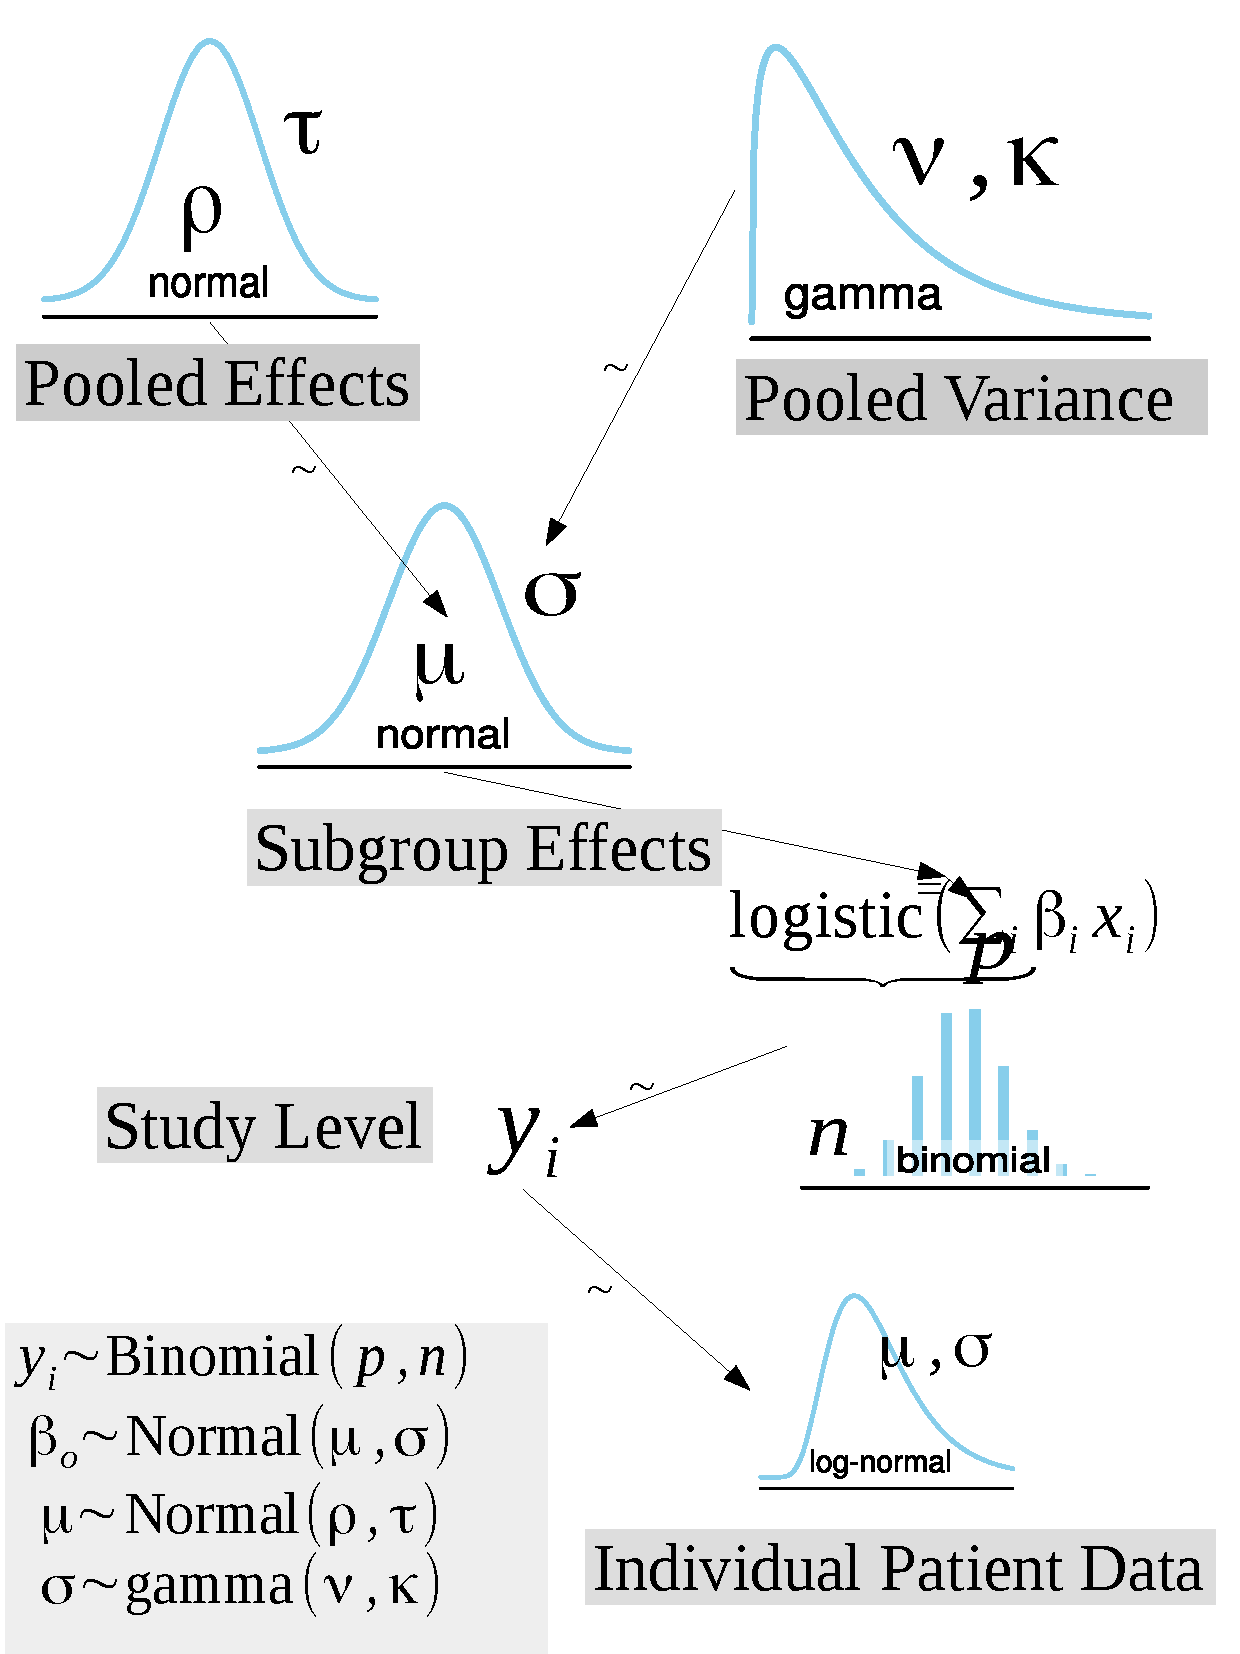
\includegraphics[width=0.35\textwidth]{Figures/DistrogramMultiLevelMetaAnalysis.pdf} 
 \caption{Multi-level meta-analysis.}
 \vspace{-10pt}
 \label{fig:MetaAnalysis}
 \vspace*{-10pt}
\end{wrapfigure}

We build a multilevel hierarchical model to pool individual patient data with continuous and 
dichotomous aggregate study-level data, clustered at the study level by followup interval and surgical 
intervention performed (Figure \ref{fig:MetaAnalysis}). Besides the three levels of hierarchical modeling just outlined 
(follow-up observations grouped by patient, patients grouped withing trials, trials within population), 
Additional hierarchical structure may be needed reconcile the substantial between-study variance in findings \cite{Andreae2015}. 
Evidence synthesis may seek to integrate continuous and dichotomous outcome measures \cite{AndreaeJohnsonAbstract2013}, since
meta-analysis requires \textit{all} available data sources \cite{Deeks2011chapter}. However, short of having access to all individual patient data, 
the integration of dichotomous outcomes and continuous outcomes is challenging with traditional software
\cite{Andreae2015, Roth2015CriticalCare}. 

\subsection*{The antithesis of complete versus no-pooling limits meta-analysis of perioperative outcomes}
To illuminate how the false dichotomy between complete versus non-pooling also limits evidence 
synthesis, we consider meta-analysis of trials with repeated observations on the outcome of interest. 
The follow-up intervals (at which perioperative outcomes are reported) 
often vary in different studies. Additionall, some studies report repeated measures, while
others only report a single terminal observation, which leads to the same issue of (a) complete pooling 
versus (b) no-pooling in evidence synthesis 
\cite{Roth2015CriticalCare}.

(a) Complete pooling:
Evidence synthesis of all effect estimates at all time points irrespective of follow-up time 
fails to consider the correlation of repeated measure. Obviously, it is usually inappropriate 
to ignore the fact that the effect estimates may depend on how long after the intervention the outcome was observed.

(b) No-pooling: Conducting separate meta-analysis for each follow-up visit would undermining the main 
strength of meta-analysis, in addition to the estimates being statistically unjustified and imprecise.

\subsubsection*{Clustering and correlations can bias clinical inferences in meta-analysis }
An even more serious bias results from failing to consider correlations 
between outcomes. Interpretation of meta-analyses, and especially Cochrane Reviews, in clinical practice 
are often reduced to "shows a significant effect" vs. "shows no significant effect". But modeling rather than
ignoring the correlations between outcomes could turn a significant effect into a non-significant effect 
(or vice versa) and the origianl model could overestimate or underestimate the variability of correlated outcomes. 
For example, assume the estimated overall relative risk (RR) is $0.8$ for an 
intervention across all studies pooled. The estimation of a $95$\% confidence 
interval of $0.55-1.15$ would lead to the inference of "no statistically 
significant effect" and thwart further attempt to study this intervention, 
while a $95$\% confidence interval of $0.7-0.9$ for the effect estimate may 
lead to widespread adoption of this therapeutic approach, with huge clinical impact.

\subsubsection*{Ecological, disease and geographic study level characteristics can influence inferences}
There are other forms of ecological bias to be considered in meta-analysis besides clustering by reported time endpoint. Geographical or 
historical settings, similar surgical procedures, or related diseases will lead to correlated outcomes in patient cohorts 
\cite{Abroug2011,Andreae2013,Andreae2015,Roth2015CriticalCare}. 
Thus, the same false dichotomy of complete pooling versus no-pooling limits meta-analysis for perioperative outcomes and hinders evidence-based 
medicine. The locations of the estimates, their precision, and the inter- and within-study variability may all differ considerably 
contingent on disease, procedure, or other study level characteristics \cite{Andreae2013,Andreae2015,Roth2015CriticalCare}.

\subsubsection*{Partial pooling across similar populations}
The principle hierarchical modeling for evidence synthesis is analogous to outcome research in general where we 
consider effects that more prominent in one trial or subgroup of the population and not as strong in another similar, but 
distinct, trial or subgroup. Examples include the meta-analyses of a treatment effect in conditions with different but 
related etiologies and the spectrum of HIV-related, idiopathic, diabetic, and traumatic chronic painful neuropathy 
\cite{Andreae2015}. Information in one subset or study population can and should inform estimates in other similar populations 
to some estimated extent in a hierarchical meta-analysis. The principle applies in other fields of medicine, e.g., critical care
\cite{Roth2015CriticalCare}, and becomes more relevant if the average effect sizes, the precision of effect 
estimates, and the inter- and within-subgroup variability differ considerably from the subgroups used to obtain 
the aforementioned findings.

\subsection*{Hierarchical modeling to improve data-intensive outcomes research}
 
Hierarchical models are thus a useful tool for analyses of
heterogeneous perioperative outcome data. This is true for meta-analysis 
of long-term studies with varied design to better inform clinical 
decisions\cite{AndreaeJohnsonAbstract2013,Spiegelhalter2004bayesian} and 
for outcomes research in our hierarchically structured contemporary health care delivery system. 
Advanced hierarchical models can be difficult to fit with traditional software but should be 
made more accessible (see letter of support by Drs. OMalley, Sacks and DiMaggio).

\subsection*{Clustering can bias estimation of confidence intervals.} To 
correctly estimate confidence intervals even in a simple Student t-test, 
we have to consider if the data are independent, which they would not be if
they are observed for the same patient multiple times. Failure to take into 
account dependence in clustered observation may lead to incorrect inferences. 
Correction to condience intervals, such as weighted jackknife methods, can 
improve matters, but such approaches are often ignored in EHR research 
and they depend on characteristics that may not hold in faceted EHR data. 

\section*{Integrating incomplete data into clustered EHR modeling}
Too often data scientists either (1) fit sophisticated models, but limit their analysis 
to complete cases, ignoring any missing or incomplete data or (2) impute the missing 
data using overly simplified models of the scientific question of interest (see letter of 
support by Dr. Mirhaji). Hierarchical modeling can synthesize the model(s) for the missingness
with the model for the outcome(s).

\subparagraph*{EHR data are not missing at random.}
Physicians chose which test to administer in order
to inform specific therapeutic decisions. Different types of data are recorded 
in different clinical settings (e.g., arterial lines may not be permissible on the 
floor, vitals are recorded in greater detail and more frequently in high dependency 
units like the ICU). In the Innovation section, we explain how both missing data 
imputation and clustering can be integrated into a single model that 
incorporates auxiliary data.

\section*{Innovation}

From about 1990 to about 2010, Markov Chain Monte Carlo (MCMC) was the most
important breakthrough for applied statistics in all quantitative subfields,
including medical research. Hamiltonian MCMC has become prominent in the 
past five years and is likely to drive the next generation of applied
statistcs that utilizes MCMC. Compared to first generation MCMC such as 
Gibbs samplers and random-walk Metropolis-Hastings, Hamiltonian MCMC converges
to the posterior distribution in fewer iterations, exhibits negligible dependence
between consecutive draws from the posterior distributions, and outputs auxiliary
information that indicates when something has gone wrong. These innovations allow
applied statisticians to fit more sophisticated models, such as hierarchical models,
and to expect results that are statistically reliable.

The \textit{Stan} project is at the forefront of the Hamiltonian MCMC revolution.
\textit{Stan} provided the first general implementation of Hamiltonian MCMC in 2012 and
incorporated two critical features that overcame the main inhibitors to its widespread
adoption. First, \textit{Stan} is almost self-tuning, so
researchers can focus on specifying their models rather than wasting time trying to
tweak algorithms they have a very limited understanding of in hopes of obtaining 
acceptable performance when estimating their models. Second, \textit{Stan} utilizes
automatic differentiation, which relieves researchers of the burden of supplying
a function that calculates the gradient of the posterior distribution with respect
to the (perhaps thousands of) parameters in their model.

Despite all these technological advances, \textit{Stan} is currently not widely used
in medical research, although it is now well-known in other subfields. Our grant
proposal is innovative in the sense that it will break down three remaining barriers
to using \textit{Stan} productively in data-intensive medical research. 

First, up until the last few months, the only way to use \textit{Stan} was to write the 
model from scratch in the Stan language, which requires considerable expertise in 
probability theory and substantial experience using \textit{Stan} in order to estimate
a model as complex as a hierarchical regression with many grouping factors. Today, it
is quite possible to use our \textit{rstanarm} package for \textit{R} to estimate
pre-written hierarchical models in the Stan language that are very general, highly
optimized, and extensively tested by Dr. Goodrich and Mr. Gabry. Thusfar, \textit{rstanarm}
has focused on applications in the social sciences and more work is needed to enhance
\textit{rstanarm} for medical research by incporating suggestions from medical researchers.

Second, although \textit{Stan} can treat missing values on continuous variables as 
additional unknowns of the posterior distribution, it is not particularly easy to do so
in the Stan language. Moreover, dealing with missing values on discrete variables is
downright tedious. By the end of the grant, we would like models provided by 
\textit{rstanarm} to handle missing data seamlessly but in a statistically appropriate
fashion. As an intermediate step, we will innovate by overhauling our \textit{mi}
package for multiple imputation of missing data to utilize the advanced model-fitting
functions provided by the \textit{rstanarm} package. Doing so will allow missing values
to be imputed in such a way that it preserves the rich grouping structure in EHR data, 
which is currently ignored by \textit{mi} and all other algorithms for multiple imputation.

Third, a variety of things can nevertheless go wrong, and it is critical that such
problems be recognized and overcome. For example, \textit{Stan}'s self-tuning is a 
work in progress and in any particular research project may require the user to tweak 
one setting. Or one reparameterization of the model may be much more computationally efficient 
than a logically equivalent one. Finally, the model may simply fail to fit the data well.
We will innovate by continuing to develop \textit{shinystan}, which is a web-application
that integrates with \textit{rstanarm} and provides a plethora of graphs to visualize the 
parameter estimates, diagnose the supplemental Hamiltonian MCMC output, and make scientific
inferences (see letter of support by Dr. DiMaggio). Without \textit{shinystan}, understanding 
the output of a complex hierarchical model would be difficult for all but the most computationally 
sophisticated medical researchers.

\section*{Approach}

We propose to further develop three interrelated software packages (\textit{rstanarm} 
\textit{shinystan}, and \textit{mi}) for the programming language and software environment 
\textit{R} so that they are reliable and well-tested. Each of these \textit{R} packages are currently available for 
free to researchers via the Comprehensive R Archive Network (CRAN) software repository. Our software development project will be guided by a multidisciplinary 
team, which will conduct its work through regularly scheduled weekly meetings and collaborate online via Github 
\cite{Chacon2009ProGit}, Google Hangouts, and email.

These software products will facilitate hierarchical modeling for data-intensive outcomes research ---
even if some of the data are incomplete --- and make it easy to visualize, diagnose, and understand the model
output. We will also promote and disseminate these innovations through presentations, graduate-level teaching, 
workshops, online tutorials, books, YouTube videos, and other publications.

\subsection*{The state of software for hierarchical modeling}

The Bayesian inference Using Gibbs Sampling (BUGS) project got its start in 1989 and has 
since grown into a family of related software such as WinBUGS (for Windows), Just Another
Gibbs Sampler (JAGS), and OpenBUGS. Bradley Carlin, a prominent Bayesian professor of biostatistics, 
\href{http://www.mrc-bsu.cam.ac.uk/software/bugs/the-bugs-project-the-bugs-book/the-bugs-book-reviews/}{stated}
\begin{quote}
MCMC freed Bayes from the shackles of conjugate priors and the curse of dimensionality; 
BUGS then brought MCMC-Bayes to the masses, yielding an astonishing explosion in the number, 
quality, and complexity of Bayesian inference over a vast array of application areas, from 
finance to medicine to data mining.
\end{quote}
Although there are many examples of BUGS models available on the internet, a BUGS model
essentially has to be written from scratch for each new research project, which is too much
to ask of many medical researchers. At the same time, it is widely known that it is all too easy to 
write a model in the BUGS \textit{language} that is infeasible for the BUGS MCMC \textit{engines} 
to sample from efficiently. In particular, BUGS models with many parameters are difficult to fit 
because BUGS typically can only update the state of the Markov chain one parameter at a time
(see letter by Drs. Kheterpal and Dutton and letter by Dr. Sacks).

Consequently, in recent years many hierarchical modelers have shifted back to essentially
frequentist estimators that choose the common parameters to maximize a (perhaps penalized) 
likelihood function that integrates out all the group-specific unknowns. Examples of this
approach include the \textit{lme4} package for R, the PROC MIXED subroutine for SAS, and
the \texttt{xtmixed} and \texttt{gllamm} functions for Stata. 

These approaches have their pros and cons. One on hand, they make multilevel modeling much more accessable to a larger number
of researchers because the user-facing functions are simple but abstract. A user need only specify the
outcome and the predictors, the grouping structure, and perhaps some options in order to estimate
a particular model that has been pre-written in a compiled language. Thus, users need not write customized 
modeling code like they would with BUGS.

On the other hand, these frequentist approaches do not provide measures of uncertainty for the
group-specific unknowns, such as intercepts and coefficients. Indeed these group-specific
unknowns are not considered parameters to be estimated but rather random variables to be
predicted. In medical treatment centers, doctors may well be interested in the implications
of a researcher's model for a particular patient, but the uncertainty in the patient-specific
unknowns cannot be easily quantified with these frequentist estimators. In addition, the 
estimated standard errors for the common parameters are obtained under the assumption that
the group-specific random variables are known. Consequently, when there are many group-specific
unknowns, the true uncertainty in the estimates of the common parameters may be understated. 
Finally, complicated hierarchical models often encounter computational problems that prevent
the optimizer from finding the maximum in the interior of the parameter space.

The \textit{Stan} language, mathematical library, and algorithms pick up where BUGS left off.
An enormous variety of hierarchical models can be specified in the Stan language, although the
researcher needs to possess considerable skill in computational statistics in order to specify
a complex model. Given a hierarchical specification, the Hamiltonian MCMC engine included in \textit{Stan}
can jointly sample from the posterior distribution efficiently, even if there are hundreds of thousands
of parameters to estimate. With MCMC estimators, both the common and the group-specific parameters
are part of the joint posterior distribution, so their uncertainty can easily be summarized by
the standard deviation of the posterior samples, credible intervals, and so forth.

What is needed now is to tack back in the direction of the \textit{lme4} package in order to
make the power of \textit{Stan}'s Hamiltonian MCMC engine available to a broader subset of medical
researchers who are interested in estimating hierarchical models (see letter of support 
by Drs. Sacks and O'Malley). This step has been partially accomplished
by the first public release of the \textit{rstanarm} R package on CRAN in mid-January of 2016. The 
\texttt{stan\_glmer} function in the \textit{rstanarm} package adopts the same syntax for specifying hierarchical
models as the \texttt{glmer} function in the \textit{lme4} package, which is a slight generalization
of the now standard R syntax for specifying models via a formula that refers to the outcome and 
predictor variables that are columns within a data.frame. The transparency of \textit{rstanarm} will 
make medical researcher more reproducible and reliable enough even for federal regulatory processes. 

For example, to specify a linear model where the intercept and the coefficient on the \texttt{x2} 
variable are allowed to vary by group, a user would specify something like \texttt{y \textasciitilde x1 + (1 + x2|g)}
where the dependent response variable $y$ is on the left of a tilde ($\sim$) operator; 
the independent terms, $x_1, x_2...$ are on the right and separated by the $+$ 
operator. Group-specific terms are distinguished by vertical bars $|$ separating expressions for design matrices from grouping factors.

Thus, the researcher need not express a hierarchical model in the Stan language in order to estimate that model with \textit{Stan}'s Hamiltonian
MCMC engine because \textit{rstanarm} comes with abstract models have already been written in the Stan language by 
Dr. Goodrich and Mr. Gabry and, of equal importance, have been tested to verify that the models work correctly. In short, 
\textit{rstanarm} combines the user-friendliness of \textit{lme4} with the 
computational efficiency of \textit{Stan} and is integrated with the other parts of the Stan ecosystem
--- all of which are open-source and free for anyone to use --- such as the \textit{shinystan} package for 
visualizing and diagnosing problems in the estimates.

Priors \textit{can} incorporate subjective beliefs or existing information about a parameter,  
which we discussed in more detail under significance \cite{carlin1997bayes}. 
Bayesian models require priors and \textit{rstanarm} by default 
adds independent weakly informative priors on the coefficients of generalized linear models, 
but more informative priors can be specified by the user. Especially in hierarchical modeling, 
regularization with priors can help convergence and improve estimates and predictions
\cite{Gelman-Hill_2014}. In \textit{rstanarm}, the user can choose from 
a broad array of prior distributions. For example, one might choose a 
Student t distribution for the intercept, which approaches the normal distribution as the 
degrees of freedom parameter approaches infinity and approaches the Cauchy distribution as the
degrees of freedom parameter approaches one. Moreover, the degrees of freedom can be estimated
in hierarchical models, which allows the data to determine what tail heaviness is appropriate.

To date, \textit{rstanarm} has only had one official release, so there are some features that are 
incompletely implemented and a trickle of small bugs have already been discovered by users, which 
may continue for some time as \textit{rstanarm} gets more exposure in different research contexts.
Nevertheless, the foundation of \textit{rstanarm} appears to be solid and it is ready to be built
upon in order to make even more sophisticated and flexible hierarchical models accessable to medical researchers.
Dr. Goodrich and Mr. Gabry stand ready to implement the models suggested by Drs. Andreae, Hall, and 
Gong, as well as the broader medical research community. One of Dr. Hall's first suggestions is to
support change-point models in \textit{rstanarm}.

\subsection*{The state of software for multiple imputation of missing data}

Multiple imputation is now an old idea that under certain assumptions about the missingness 
mechanism(s) serves as a first step toward statistically justified inferences when there
are missing data. First, the researcher uses a model or sequence of models to impute values for 
each observation where the data were originally missing. This process is repeated multiple times
in order to obtain several completed data sets. Second, the researcher analyzes all of the 
completed data sets as if the data were fully observed from the outset and applies some rules to
combine the estimates from the several completed datasets.

Multiple imputation is not ubiquitous in applied research, although it is now fairly commonplace
in large part due to the availability of functions in Stata and in \textit{R} packages that try
to automate this two-step process as much as possible. However, the open secret of multiple
imputation software is that the models used to impute values in step one are very simplistic
compared to the models that are often fit to the completed data in step two. In other words,
the imputation models essentially assume the data are a simple random (albeit incomplete)
sample from a population, while the substantive models often try to exploit the obvious
grouping structure that exists in many data-generating processes, such as EHR. As a result,
the imputation process tends to dilute the group structure that is essential to the analysis.

There are two major imputation algorithms. One assumes that all of the variables are jointly
multivariate normal and estimates its mean vector and variance-covariance matrix via an
iterative process that draws values from a conditional multivariate normal distribution that
conditions on all the observed data for each observation. This approach is simple, but is 
not theoretically appropriate for binary or categorical data, which cannot be generated as
part of a multivariate normal. Nevertheless, many researchers use this algorithm even when
their variables are largely categorical on the grounds that doing so is better than not
imputing the missing values at all.

The second major imputation algorithm specifies a sequence of conditional distributions
where each model in the sequence pertains to the conditional distribution of one variable with
missingness given (some subset of) the other variables. When each model is estimated, imputed
values are drawn from a univariate conditional distribution that can be tailored to each 
variable depending on how it is measured. Thus, the second approach avoids the embarassment
of imputing continuous values for binary or categorical variables but suffers the embarassment
that the sequence of conditional distributions generally do not imply any valid joint 
distribution over all the variables with missingness. Also, if there are many variables with
missingness it is very tedious for users to specify a conditional model for each incomplete
variable.

The \textit{mi} package takes the latter approach but uses simplistic imputation models that 
ignore the grouping structure that user may know exists in the data-generating process. As
an initial step, we would like to reformulate the \textit{mi} package so that is uses the
models in the \textit{rstanarm} package to impute. Hamiltonian MCMC is generally too slow
for this task when there are many variables with missingness, but \textit{Stan} also includes
some much faster algorithms that are intended to provide draws from a reasonable approximation
to the posterior distribution. When this initial step is completed, \textit{mi} will be able
to quickly impute missing values from a model that takes into account, rather than ignores,
the same grouping structure that the researcher plans to exploit when the substantive model
is estimated on the completed data sets.

Over the longer term, we would like to include models in the \textit{rstanarm} package that
simultaneously model the missing values, the missingness mechanism, and the outcome of 
interest, which typically would include some specification of the grouping structure. This
approach implies a well-defined joint posterior distribution of the model parameters and 
the unknown data and thus should yield estimates and predictions that are not only statistically
justified but also more precise.

\subsection*{Heterogeneous and incomplete clinical data may limit prediction and implementation.}
Variables with strong predictive power may not be recorded for all patients 
or may be missing for the time window needed for prediction, which is a critical limitation 
in the development of prediction algorithms and implementation of the 
therapeutic interventions (see letter of support by Dr. Mirhaji). 
Yet, incomplete data are the hallmark of EHRs. 
Hierarchical models for incomplete data give valid estimates 
\textit{if and only if} the missingness mechanism is ignorabe, which is to say that the parameters 
for the missing data mechanism are indpenent from the parameters in the main model for the 
outcome, and the data are either missing at random (MAR) or Missing Completely At Random 
(MCAR) \cite{Rubin1976}. Indeed, these assumptions are unreasonale for EHRs. In our example, only 
significant respiratory co-morbidity and symptoms will prompt physicians to request arterial blood gases (ABG). Trying to 
impute missing ABG data using traditional multiple imputation algorithms would hence lead to biased 
imputations. Imputation using auxiliary data can help overcome this limitation, as outlined below.

\subsection*{Auxiliary data can be used to impute incomplete medical records.} 

\begin{wrapfigure}{l}{10cm} 
 \vspace{-25pt}
 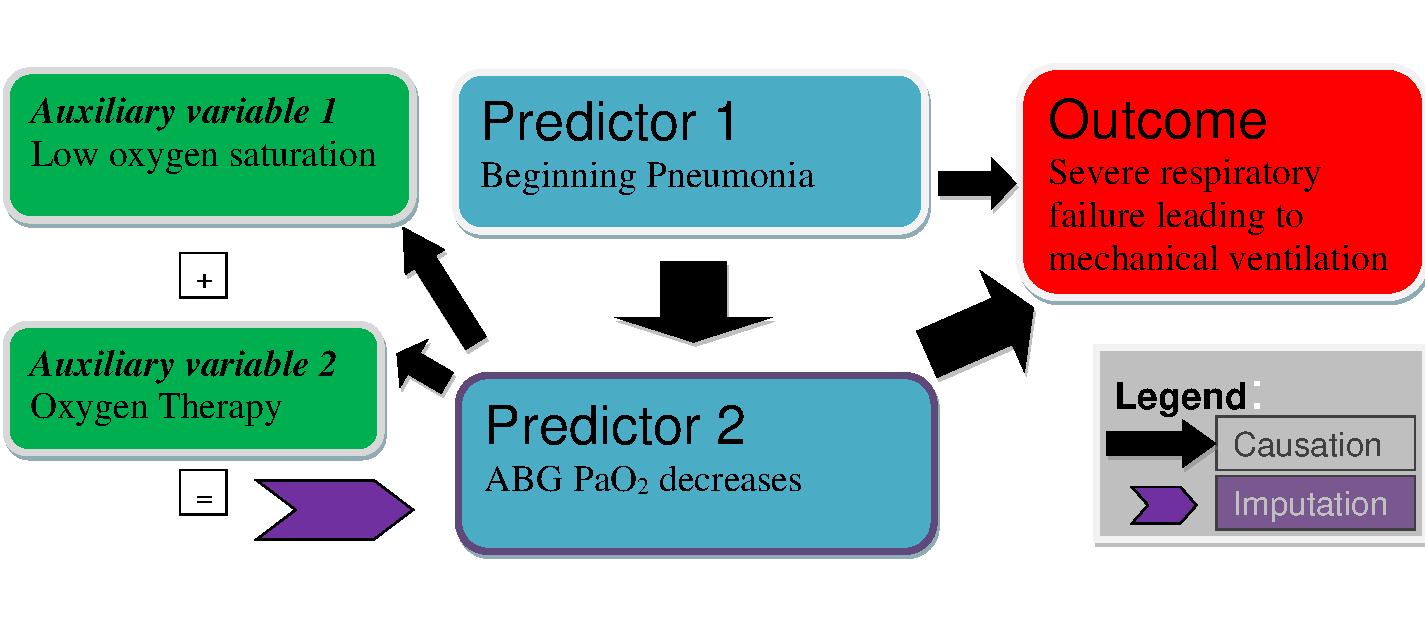
\includegraphics[scale=0.4]{Figures/Bayesian_imputation.pdf}
    \vspace{-20pt}
  \caption{Auxilliary data to impute missing information}
   \vspace{-15pt}
   \label{fig:Imputation_fig}
\end{wrapfigure}

Auxiliary data are additional information available in the form of variables known 
to be correlated with the missing data of interest 
\cite{Hall_25389642,Daniels24571539}. Figure \ref{fig:Imputation_fig} 
illustrates how we can impute incomplete data from auxiliary information 
\cite{Ibrahim2001auxilliaryImputaton,Schomaker23873614}. We know pneumonia 
impairs oxygenation, by causing respiratory failure, for example. If 
arterial $PaO_2$ (oxygen tension) is missing because arterial blood 
gases (ABG) have not been obtained, we can impute the incomplete data 
from oxygen therapy and/or peripheral oxygen saturation\cite{Hall_25389642}. 
This approach avoids the perils associated with missing at random (MAR) 
assumptions, when fitting a non-ignorable missingness model \cite{Wang_20029935}. 
Adding auxiliary variables not included in the main model for multiple imputation, 
in other words using additional information that is correlated with the missing 
outcome is an emerging approach to help correct bias 
\cite{Meng1994, Collins_11778676, Rubin1996}, often relying on 
Bayesian methods \cite{Daniels2008, Schafer1997}. Joint hierarchical 
modeling, including auxiliary data to impute incomplete patient records, 
will improve the prediction model and facilitate the implementation of the 
prediction algorithm \cite{Hall_25389642}.

\subsection*{The state of software for visualizing MCMC output}

Almost all MCMC software has some capability to make graphs from MCMC output. But none are as
user-friendly or as capable as \textit{shinystan} for exploring and troubleshooting the output of 
hierarchical models.

\begin{wrapfigure}{l}{.6\textwidth}
  \vspace{-10pt}
 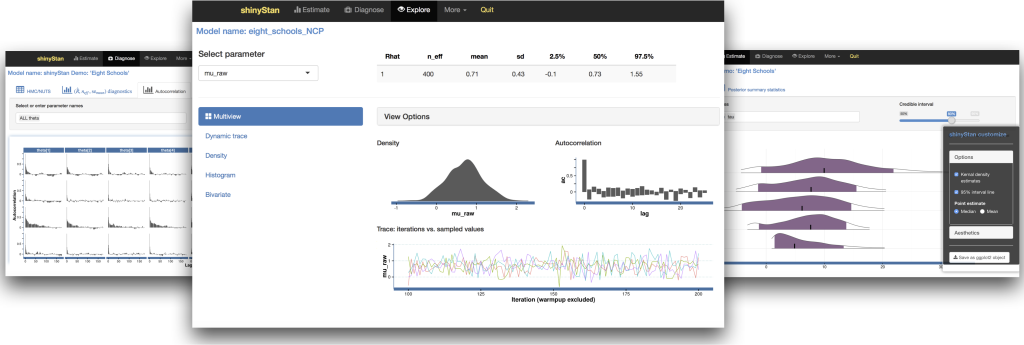
\includegraphics[scale=1.2]{Figures/shinystan.png}
  \vspace{-12pt}
  \caption{\textit{shinystan} interface}
    \label{fig:shinystan}
 \vspace{- 14pt}
\end{wrapfigure}

The interactive user interface of \textit{shinystan} shown in Figure \ref{fig:shinystan} 
demonstrates how easy it is to do posterior predictive checks of the model against the
observed data, which are routine if the model was estimated by any of the
functions in the \textit{rstanarm} package. If a hierarchical 
model fails to converge, ascertaining why is crucial to troubleshooting. \textit{shinystan} 
is already unmatched in combining ease of interactive graphical exploration 
with sophisticated graphical rendering to explore correlation between parameters, autocorrelation
in the draws, the number of steps that the Hamiltonian MCMC sampler took on each iteration and 
many other convergence diagnostics.

Although \textit{shinystan} is already available on \href{https://cran.r-project.org/web/packages/shinystan/index.html}{CRAN} 
and is a fully functional \href{https://www.youtube.com/watch?v=X31xqNHcvQs}{package}, it
will need to undergo considerable improvements of the interface and under the hood during this project. Posterior predictive 
checking is one area where the need for additional options and functionality. We also want to expand the existing collaborative 
model sharing via the internet. We will not only further develop \textit{shinystan} 
to make it more robust and scale it to work faster for larger models and data sets. We will continue to develop novel graphical 
methods to assess model convergence with a special focus on hierarchical modeling. Finally, a
major long-term goal for \textit{shinystan} is to be able to save the \textit{R} code that 
generates each of these graphics. When that capability is added, users will be able to
include the plot-generating code in their \textit{R} scrips so that the graphics can 
easily be updated whenever new observations are added to a data set or when the model is tweaked.

As we further develop the interface we will place special emphasis on the concept of affordance in our "intuitive" 
design of the \textit{shinystan} graphical user interfaces, e.g., in employing strong visual clues, provide clickable buttons and tabs, sliders, and other 
hands on interactive controls \cite{NormanAffordances1999}. Active exploration by \textit{shinystan} users will reveal nested and sequential 
affordances, for example, print options appear only in context, say when the cursor moves over the output button of a graphic, 
avoiding visual clutter on the screen with irrelevant information \cite{Mcgrenere2000affordances}. We will rely on user 
feedback to optimize the practical utility of \textit{shinystan's} implementation and user interface.

\section*{Project scope and goals}

In summary, we propose to further develop, test, and harden our three software packages: \textit{rstanarm}, \textit{shinystan}, and \textit{mi}.

\subsection*{\textit{rstanarm} for accessible hierarchical modeling}
The first proposed software package \textit{rstanarm} allows data scientists to specify the most common applied hierarchial regression models 
and estimates them via \textit{Stan}'s implementation of Hamiltonian MCMC algorithm. Researchers do not
need to understand the underlying intricacies (e.g., auxiliary parameterizations) that have been implemented in order to accelerate convergence and 
do not need to build complicated data structures to keep track of group indexing. \textit{rstanarm}'s syntax makes hierarchical model building easy
because it is the same as the familiar notation for specifying models in \textit{R} and popular \textit{R} packages such as \textit{lme4} \cite{lme4}.
We will add additional models to \textit{rstanarm} so that it is the premere tool for hierarchical modeling in medical research.

\subsection*{\textit{shinystan} for interactive graphical exploration and diagnosis of MCMC output}  
The second \textit{R} package, \textit{shinystan}, is a graphical user interface for interactively exploring any model estimated by MCMC. 
\textit{shinystan} provides multidimensional visual tools for any analyzing high-dimensional MCMC output, particularly for 
\textit{rstanarm}. \textit{shinystan}'s web-application interface is user-friendly and requires minimal training for novices.

\subsection*{\textit{mi} for multiple imputation of missing data}
The third \textit{R} package, \textit{mi}, performs multiple imputation of missing data by specifying a simplistic model 
for each incomplete variable. We propose instead using the models provided by \textit{rstanarm} to provided the basis for
the imputations, which would allow us to specify the group structure that is evident in EHR data. Ultimately, we 
propose enhancing \textit{rstanarm} so that it can estimate models in a statistically principled way, even when some of
the data are incomplete.

\subsection*{Prior work in statistical software development and data-intensive outcomes research}
 
Dr. Andreae published several meta-analyses and synthesized the evidence 
from clinical trials by pooling aggregate and individual patient data, when 
published results were insufficient for classical meta-analysis 
\cite{AndreaeJohnsonAbstract2013, Andreae2013, Andreae2015, Carter2015, Atchabahian2015}. Dr. Andreae, Hall, and 
collaborators used the software \textit{rstanarm} and \textit{shinystan} to build a multilevel 
hierarchical model to investigate health care disparities and quality of 
anesthesia delivery in the large National Clinical Outcomes Registry maintained 
by the American Society of Anesthesiology \cite{AndreaeWhite2015}. 

Dr. Hall has also published on missing data 
imputation \cite{Hall2009a, Wang_20029935, Wang_20029935} and is internationally 
recognized for the development and application of change point models in 
epidemiology and surveillance \cite{Hall2000, Hall2001, Hall2003bayesian, Hall2009, Hall2015}. 
More recently, Dr. Hall has played a major role as the lead statistician 
for the World Trade Center (WTC) Health Program at the Fire Department 
of the City of New York, supervising data analyses based on medical 
records \cite{Aldrich2010, Hall2015, Zeig-Owens2011}.

Dr. Goodrich built the current version of the R package \textit{mi} as a postdoctoral researcher working with
Dr. Gelman \cite{miCRAN} who is internationally recognized as a leader in Bayesian statistics, hierarchical 
modeling, and data imputation \cite{Gelman1998notasked, Gelman2001imputation, Hoffman2014, Gelman-Hill_2014}. 
Dr. Gelman oversees \textit{Stan}\cite{Stan_Software_2014} project, which which provides the foundation for the 
proposed work and Dr. Goodrich has been one of several core developers supplying that foundation since 2011.  
Dr. Betancourt is also a core developer of \textit{Stan} and a consultant on this grant who has special expertise in the differential 
geometry underlying the Hamiltonian MCMC algorithm in \textit{Stan} that allows for automated tuning heuristics
\cite{BetancourtGeometry2016}.

Dr. Goodrich is now the maintainer of the \textit{rstan} R package and the \textit{rstanarm} package that extends
it, which was written entirely by Dr. Goodrich and Mr. Gabry. Mr. Gabry is the maintainer and essentially the
sole author of the \textit{shinystan} R package.

Dr. Gong's ongoing NIH funded trial to predict and improve 
respiratory outcomes after intubation based on real time 
electronic medical records is just one of many examples of her 
leading role in applied data driven outcomes research 
\cite{Gong2005, Gong2010, Gajic2011, Yu_24970344, Kor2014}. 

\subsection*{The trajectory leading to the development of \textit{rstanarm} and \textit{shinystan}} 

\begin{wrapfigure}{l}{0.6\textwidth} 
 \vspace{- 15pt}
    \centering
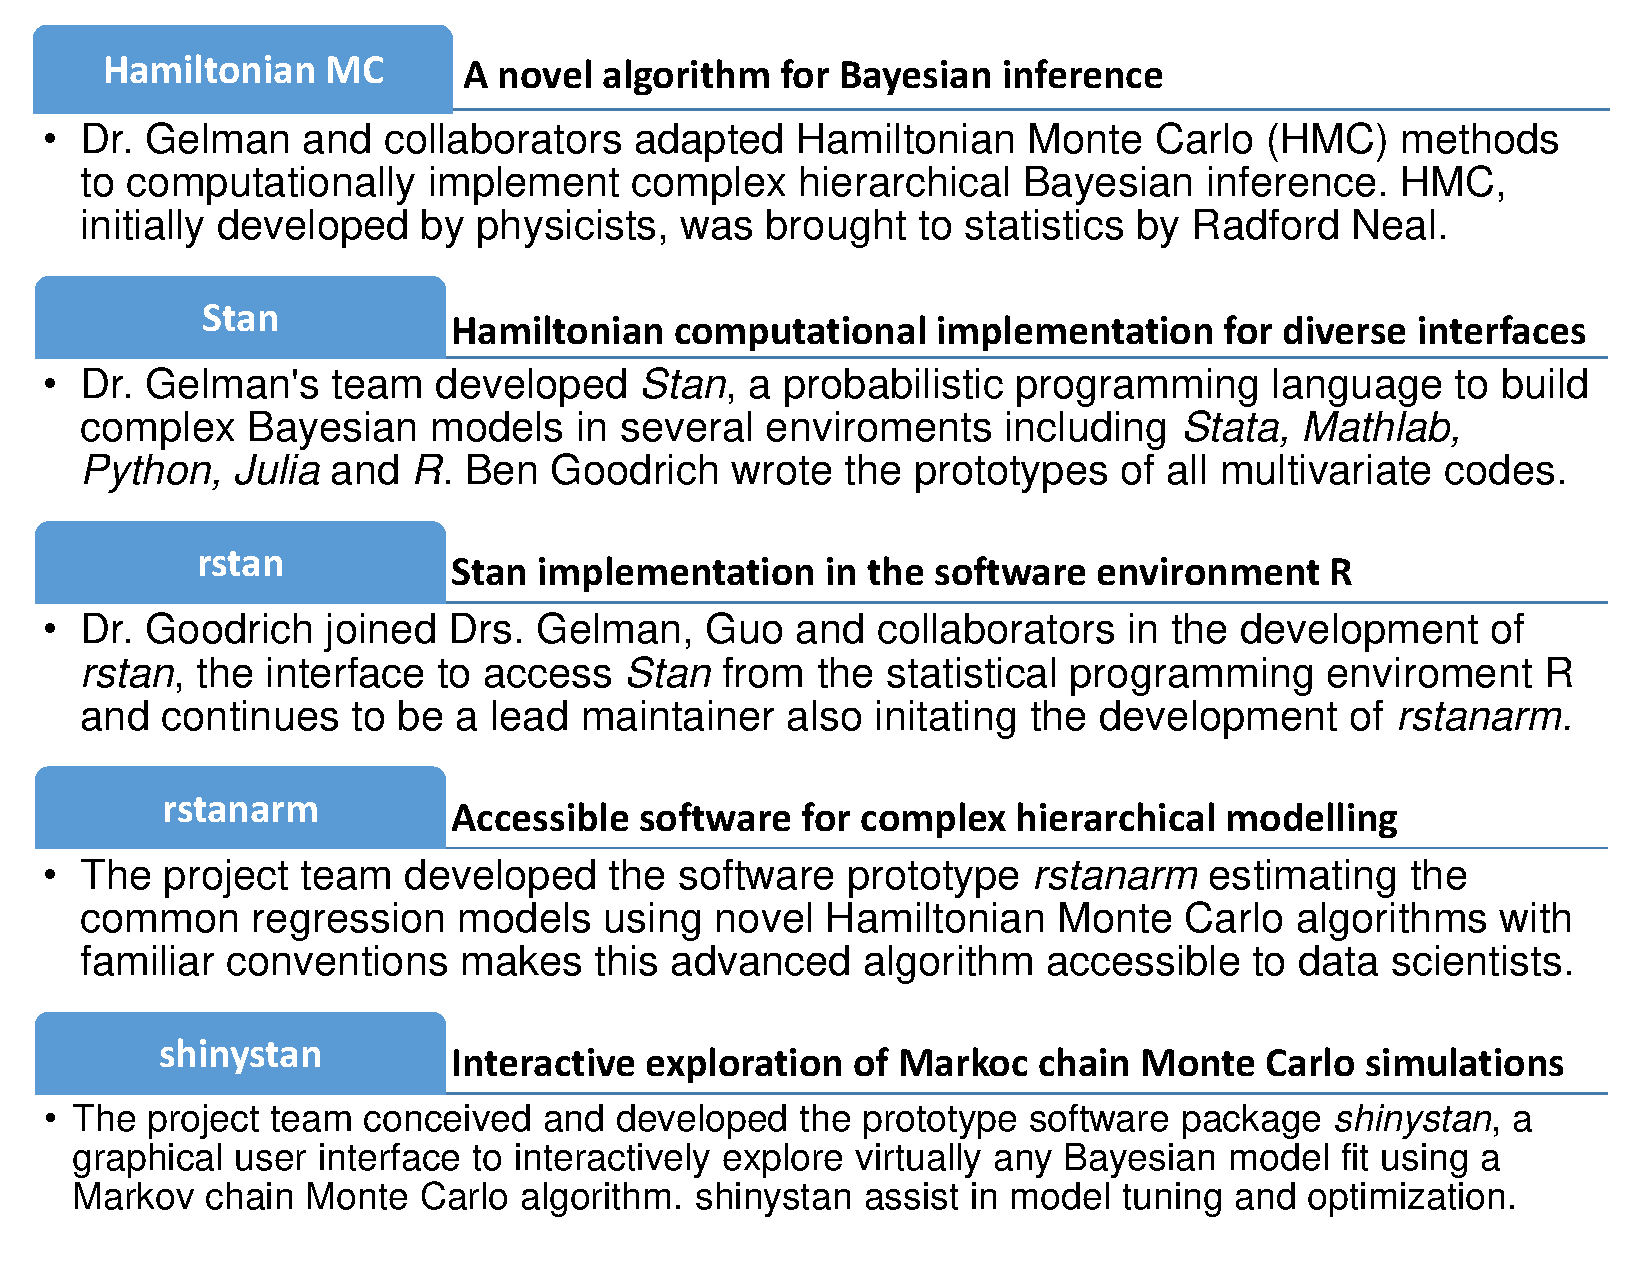
\includegraphics[width=0.6\textwidth]{Figures/SoftwareTrajectory.pdf}
  \vspace{-32pt}
  \caption{Software development trajectory}
    \label{fig:trajectory}
 \vspace{- 15pt}
\end{wrapfigure}

The National Institute of Health, the Center for Disease Control and the National Science Foundation, 
(NIH: 5R01GM074806, 5KL2TR001071, UH2-HL125119,  CDC: U01 OH010711-01 and NSF: SES-1205516) were among the many 
federal institutions funding Stan \cite{Stan-manual:2015} development and its empirical applications.
The work proposed here is thus a direct continuation of the aforementioned work that developed and implementing 
ground-breaking algorithms that are capable of estimating complex hierarchical models. Figure \ref{fig:trajectory} to the above left 
outlines the trajectory that led to the current project proposal.

\section*{Collaborative software development and computer resources}
We will follow accepted best practices, proven methods, and industry standards for open-source software design, construction and implementation.
For example, when building \textit{Stan} and its ecosystem of interfaces, we have trie to follow the rules of clarity, composition, separation, 
simplicity, transparency, etc. set form by Raymond \cite{Raymond2003art}.

\subparagraph*{The source code of \textit{rstanarm} and \textit{shinystan} are managed through the Git version control system}
\cite{Chacon2009ProGit} via the online software repository \href{https://github.com/}{Github} for integrated issue tracking, 
progress milestones, and code history tracking \cite{loeliger2012version}. We will use the Git process \cite{Driessen2010successful}, 
as we did sucessfully for the development of \textit{Stan} \cite{Stan-manual:2015}. This  process is based on collaborative code review, 
where new features or functions are developed creating a branch; proposed changes and additions are discussed following a pull request on 
Github. The ability to write to the repository is restricted to the core team, while any user can propose patches to address software 
bugs or suggest improvements. Further commits are commonly added after substantial feedback and testing before merging the branch.  
On Github, altered syntax is highlighted and changes are transparent and revertible, making collaborative software development easier. 
Github's distributed structure implies that everybody cloning the repository generates a backup. We prototype and test additional 
functions and features before inserting them in any package update.

The development, extension, testing and maintenance of our packages is a collaborative effort by our multidisciplinary team with 
communication and input taking place in several venues. Public user groups and discussion are archived and freely accessible. 
Confidential deliberations, (e.g., regarding grant related matters), are held in private restricted groups. We will hold weekly video 
conferences to prioritize issues and discuss progress.

\subparagraph{Montefiore Medical Center and Columbia University will provide the computer cluster access} required for the computationally intensive 
models and provide server space to house webpages. Clinical Research Informatics at Montefiore will provide scale-able 
remote access via a secure virtual private network to up to 32 Xenon Intel processors in parallel on a windows virtual machine with up to 
128 GB RAM to meet the variable needs of the project throughout the course of the grant. 

As also discussed under the subsection on human subject protection and in the letter of support by Dr. Mirhaji, some of the data sets to 
be used for this project cannot be completely de-identified. Rather, they are 'limited data sets' that still contain some patient 
identifiers (e.g., age in years or zip code). Hence, the computer clusters housing the data and 
any computers that we use to analyze the data have to be compliant with the Health Insurance Portability and Accountability Act (HIPPA. 
Clinical Research Informatics at Montefiore will house any data set falling under HIPPA and 
guarantee compliance with relevant federal data safety and privacy regulations (see letter by Dr. Mirhaji). 

\section*{Dissemination and unimpeded utilization of the products of this project}
The goal of this project is to encourage widespread adoption of cutting-edge 
hierarchical modeling for data-intensive outcomes research by clinical scientists and to support the use of our 
open source applications. The software developed for this grant will hence all be incorporated into the public repository CRAN, 
of the open-source R Project for Statistical Computing. Our source code and documentation 
will be distributed under the least restrictive open-source licensing terms possible: R's licensing is \textit{copyleft} under the 
GNU General Public License. \textit{Copyleft} refers to licensing arrangement that allow for the software can be used, modified and/or 
distributed freely on condition that anything derived is bound by the same condition. The benefits  are that our software 
(1) will be freely available to researchers and the general public, including for commercial use, 
(2) shall remain freely available to the public and may be freely extended, 
(3) may be incorporated into the other tools that also are licensed under the same terms, 
(4) can be maintained if the original developers are no longer able to, and
(5) can be enhanced based on user-provided feedback for bug-fixes, examples, and enhancements.

\subsubsection*{Prior team experience and exposure in statistical and quantitative teaching and dissemination}
Our project team have ample experience in teaching, publishing, and promoting software. The Co-Principal Investigators teach 
in graduate programs focused on teaching quantitative skills to social science and biomedical audiences. 
Our workshops on statistical and research methods are sought after, and we have been invited to national and international statistical and  
biomedical meetings. Our team presented workshops at a wide spectrum of scientific and statistical meetings ranging from clinically oriented 
conferences like the Annual meeting of the American Society of Anesthesiologists to \href{https://www.youtube.com/watch?v=pHsuIaPbNbY}{machine learning venues} 
to the Annual Conference on Neural Information Processing Systems (NIPS). Dr. Gelman maintains a very popular \href{http://andrewgelman.com/}{blog}. 
Presentations and products by our team have been featured on \href{https://www.youtube.com/watch?v=X31xqNHcvQs}{YouTube} and 
\href{http://thinkinator.com/2016/01/12/r-users-will-now-inevitably-become-bayesians/}{blogs} by others.   

\subsubsection*{Books, tutorials, workshops lectures and outreach to disseminate hierarchical modeling}
Throughout the duration of the project we will disseminate the software packages in tutorials, workshops, lectures, books and other forms 
of outreach. In particular, we will offer hands-on workshops at national and international for small groups based on our applied use cases 
as outlined also in the budget justification. These will be interlinked and supported by online material, for 
example YouTube videos \href{https://www.youtube.com/watch?v=pWow8Qe1snQ}{promoting} or 
\href{https://www.youtube.com/watch?v=pHsuIaPbNbY}{explaining and motivating} the algorithms underlying \textit{Stan}. We will make 
detailed \href{http://mc-stan.org/documentation/}{technical} and practical tutorials and 
\href{https://cran.r-project.org/web/packages/rstanarm/vignettes/aov.html}{vignettes} available online, interspersing code, graphics 
and detailed step-by-step explanations using \textit{R's}  \href{http://rmarkdown.rstudio.com/}{R Markdown \- Dynamic Documents for R}, 
blogs, for example our \href{http://andrewgelman.com/}{blog} on Statistical Modeling, Causal Inference, and Social Science. In addition, 
\textit{Stan} will be featured in the next edition of \cite{Gelman-Hill_2014}.

\subsubsection*{Mechanisms for incorporating feedback and user reported corrections into the software.}

We already have very active \href{https://groups.google.com/forum/#!forum/stan-users} {user groups} around \textit{Stan} and 
with frequent online and face-to-face \href{http://www.meetup.com/bda-group/}{meetings}. We will incoporate more of
\textit{rstanarm} and \textit{shinystan} in the future to to discuss implementation issues, engage advanced users in the development of 
our packages and/or in designing courses around our models and software, but in particular to solicit their feedback. The user 
forums have served also to assist novices in implementing their models in our software.
Like our existing \href{https://github.com/stan-dev/example-models/wiki}{Wiki} on Github for \textit{Stan}, we will 
take full advantage of the functionality of GitHub for engaging users in collaborative software development \cite{loeliger2012version}, 
including further development of the \textit{rstanarm} and \textit{shinystan} 
\href{https://github.com/stan-dev/rstanarm/wiki}{Wikis} and discussion of \href{https://github.com/stan-dev/rstanarm/issues}{issues} with users.

\section*{Timeline and potential problems}

\begin{wrapfigure}{l}{0.7\textwidth} %this figure will be at the right
 \vspace*{-12pt}
    \centering
  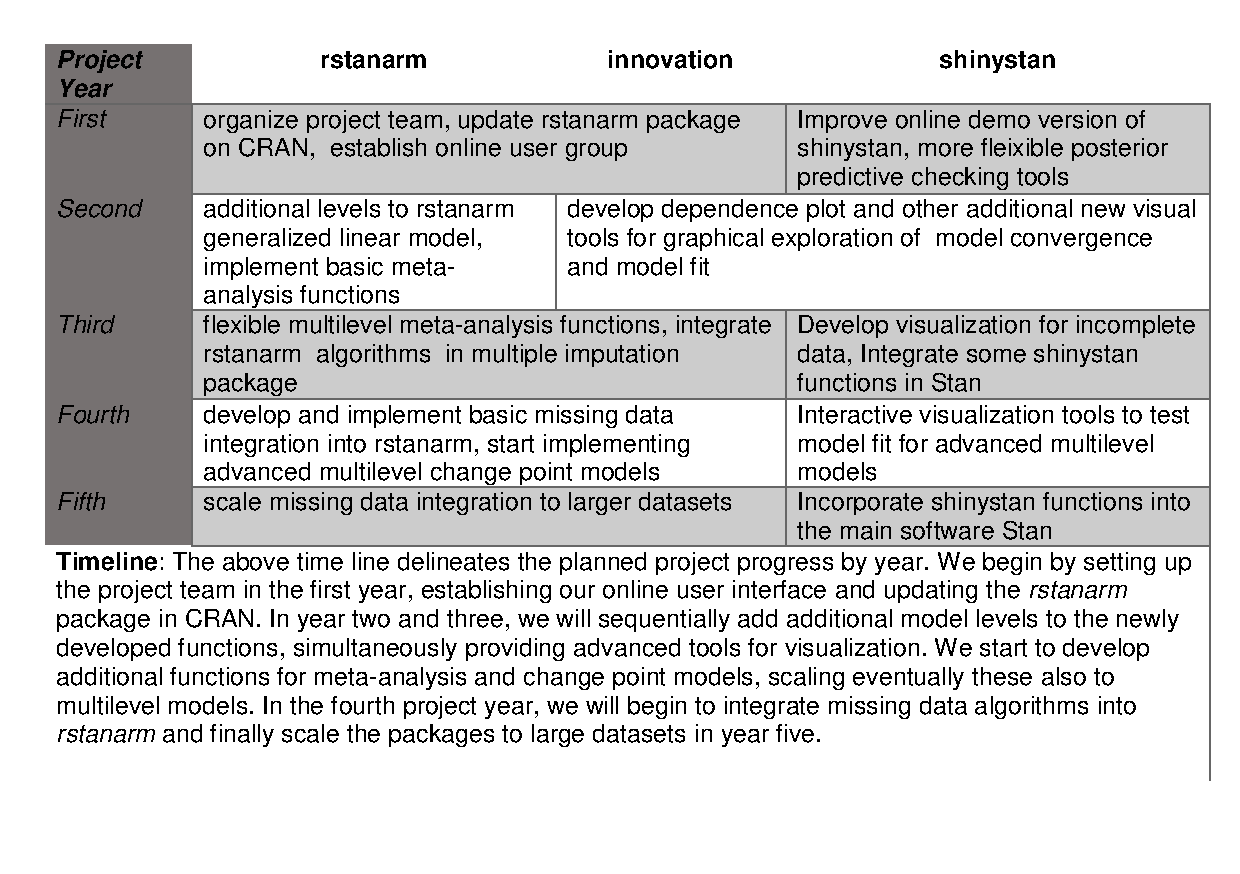
\includegraphics[width=0.7\textwidth]{Figures/Timeline.pdf}
 \vspace*{-15pt}
\end{wrapfigure}

The Timeline delineates the planned project progress by year. We begin by setting up the project team in the first year, 
establishing our online user interface and updating the \textit{rstanarm} package in CRAN. In year two and three, we will sequentially 
add additional models and provide advanced tools for visualization. We start to develop additional functions for meta-analysis and 
change-point models, scaling eventually these also to multilevel models. In the fourth project year, we will begin to integrate 
missing data algorithms into \textit{rstanarm} and finally scale the packages to large datasets in year five.

Some colleagues are reluctant to make powerful statistical tools accessible to the novice users that do not understand them. We counter 
however that the simplicity of the \textit{rstanarm} syntax will allow novice users to learn to specify more realistic models by 
making the underlying hierarchical model structure more transparent.  \textit{rstanarm} will also allow outcomes research to be 
more transparent and reproducible. Finally, \textit{shinystan} will contribute to the ease with which advanced hierarchical models and MCMC 
results can be shared, questioned, and discussed.

\newpage 
%----------------------------------------------------------------------------------------
%	BIBLIOGRAPHY
%----------------------------------------------------------------------------------------

\newpage

% \nobibliography{K01_bibliography_24Feb15} % to not print a bibiography at the end.
\bibliography{Bibliography/bibliographyBD2K} % the file name cannot contain spaces
\bibliographystyle{Bibliography/nihunsrt} % Use the custom nihunsrt bibliography style included with the template

%----------------------------------------------------------------------------------------

\end{document}

\subsection*{Fast and flexible hierarchical modeling for realistic data-intensive outcomes research }
% FIXME: Instructions say that any tables and figures must not be previously published
\begin{wrapfigure}{l}{.3\textwidth}
  \vspace{-15pt}
 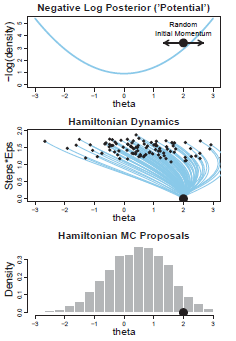
\includegraphics[scale=0.85]{Figures/Hamiltonian.png}
  \vspace{-14pt}
  \caption{Hamiltonian MCMC}
    \label{fig:Hamiltonian}
 \vspace{-16 pt}
\end{wrapfigure}

The \textit{rstanarm} package utilizes \textit{Stan}'s implementation of Hamiltonian MCMC. Figure 
\ref{fig:Hamiltonian} reproduces Fig 14 in Kruschke \cite{Kruschke_Book_2014} to illustrate how 
\textit{Stan's} Hamiltonian MCMC algorithm achieves much greater efficiency by using randomly
drawn momentum to determine the next proposed draw from the posterior distribution. The current proposal's 
higher momentum (black dot) is indicated in the top panel. The middle panel illustrates how their 
momentum along with the gradient steers random samples to the mode of the posterior distribution (shown in lower 
panel) with the correct probability. % FIXME: I am not sure this is sufficiently clear from the figure alone

\section*{Software Specification}

\subsection*{rstanarm allows for simple specification of complex hierarchical models}

\begin{wraptable}{l}{0.51\textwidth}
 \vspace*{-17pt}
 \footnotesize

\begin{tabular}{@{}
>{\columncolor[HTML]{EFEFEF}}l l@{}}
\toprule
\textbf{Function Call} & \textbf{Underlying process in \textit{rstanarm}}                        \\ \midrule
stan\_aov               & User interface for simplified model specification  \\
stan\_lm               & Parsing linear model specification \\
stan\_lm.fit           & Workhorse function to call pre-comiled \textit{Stan} model  \\
lm.stan                & Pre-compiled optimized model written in \textit{Stan}                   \\ \bottomrule
\end{tabular}

 \vspace*{-7pt}
 \caption{Handing down model specification and data}
 \label{ProcessTable}
 \vspace*{-12pt}
\end{wraptable}


\subsubsection*{A suite of pre-compiled \textit{Stan} programs allows for a simple call to sophisticated modeling functions.} 
\textit{rstanarm} already implements many generalized linear 
models with and without group-specific terms. We wrote and optimized several models 
in the probabilistic programming language \textit{Stan} that are
pre-compiled in \textit{rstanarm}. Users can now build hierarchical models via simple high-level functions. 
We take an ANOVA model as an example in Table \ref{ProcessTable}, the wrapper function $stan\_aov$ parses the 
model specification and hands the data and specification of priors (or their defaults) to $stan\_lm$ and 
then to a lower-level workhorse function, $stan\_lm.fit$, which in turn 
calls the pre-compiled and optimized \textit{Stan} model specified in 
$lm.stan$. The the Hamiltonian Monte Carlo output is returned in reverse order
through these functions to the data scientist in a list that is convenient 
for analysis, plotting, and other post-estimation functions.

The $stan\_lm$, $stan\_glm$ and $stan\_glmer$ functions are similar in syntax to the R functions $glm$ 
and $glmer$ but rather than performing maximum likelihood estimation of classical generalized linear models, 
\textit{rstanarm} emphasizes full Bayesian estimation via Hamiltonian Monte Carlo. If "weakly informative" 
priors are chosen in simple models, the posterior means will tend to be very similar to classical frequentist point 
estimates \cite{Gelman-Hill_2014}. However, \textit{rstanarm} uses the same user-friendly interface to estimate 
sophisticated hierarchical models that are too complicated for classical frequentist inference.

\subparagraph*{Further hardening, expansion and integration of \textit{rstanarm}}
While \textit{rstanarm} delivers some functionality for data scientist and is already available from 
\href{https://cran.rstudio.com/web/packages/rstanarm/}{CRAN}, much of this project will be devoted to hardening existing functionality, 
expanding functionality, and integrating functionality from other R packages. We need to incorporate user feedback, weed out 
possible bugs, and include many more functions and advanced models, such as change-point models \cite{Hall2000}. Specifically, 
we want to work on a more seamless integration with our \textit{R} package for multiple imputation of missing data 
\href{https://cran.r-project.org/web/packages/mi/index.html}{\textit{mi}}.

\subsection*{shinystan for interactive intuitive graphical exploration of MCMC output}
We propose to further develop \href{http://andrewgelman.com/2015/03/02/introducing-shinystan/}
{\textit{shinystan}} \cite{GabryISCB2015,shinystan} as an interactive graphical user interface to explore virtually any Bayesian model output, 
yet optimized for \textit{Stan}. Implemented in in \href{http://shiny.rstudio.com/}{\textit{Shiny}}, \textit{shinystan} is an R package for 
interactive web applications \cite{shinystan-software:2015,shinystan}. Data scientist already use generic extractor functions such as print() and coef(), 
but often lack a suitable method for extracting an interesting result from the model fit and hence have to resort to 
writing tedious customized code. Important model diagnostics (e.g., influence() to assess  homoscedastic residual errors) 
are not developed even for classical multi-level models \cite{Galecki2013linear}.

\begin{wraptable}{l}{0.65\textwidth}
 \vspace*{-7pt}
 \footnotesize

 \begin{tabular}{@{}
 >{\columncolor[HTML]{EFEFEF}}l l@{}}
 \toprule
 \textbf{Object} & \textbf{Increasingly informative object characteristics} \\ \midrule
 MCMC & raw data from Markov chain Monte Carlo chains \\ \midrule
 rstan & structured embedded model information (\textit{Stan} code, parameter names...) \\ \midrule
 rstanarm & accessible aggregate derived statistics (coefficients, SE, fitted, residuals) \\ \midrule
 shinystan & detailed user-friendly model meta-data, posterior predictive draws... \\ \bottomrule
\end{tabular}
 
 \vspace*{-7pt}
 \caption{Progressive enrichment of object characteristics in \textit{shinystan} }
 \label{ObjectCharactersitics}
 \vspace*{-17pt}
\end{wraptable}

Data scientists certainly lack good tools for graphical exploration of MCMC output. The graphical rendering of the plots in \textit{shinystan} 
utilizes the superb graphical package \textit{ggplot} by Hackley Wickham. 
We will develop function calls to render the code generating customized \textit{shinystan} graphical and numerical 
output, to allow users to integrate these directly into reports generated with markdown in R through the \textit{knitr} 
package. We will develop additional diagnostics in \textit{shinystan} to optimize model convergence, explore unexpected parameter 
correlations, and assess the correctness of the model specification with (a) residual diagnostics, e.g., for continuous 
covariates, a scatterplot of residuals versus covariates and (b) influence diagnostics.

\subparagraph{The automation of many data exploration processes in \textit{shinystan}} saves time, 
but implies the extraction of the meta-information about the model and 
its parameters as detailed in Table \ref{ObjectCharactersitics}. Data scientist working with the raw draws from the MCMC output 
have to extract, manage and program a plethora of details to explore higher level structure and statistics of their output. 
As we move from the MCMC output (raw draws from posterior
distributions) to the user-facing output object structures become richer with model-specific 
information (e.g., \textit{Stan} code). The user-friendly \textit{rstanarm} 
package contains even more accessible information that is derived from the original function call. 
Finally, the interactive web based tool \textit{shinystan} extracts and processes much more meta-data to 
facilitate access to the required fit object elements for visual exploration and troubleshooting.

\subparagraph*{Improving and hardening \textit{shinystan}}

\subparagraph{Improving the graphical representation of shrinkage in hierarchical models for meta-analysis.} Forest plots display the effect estimates of individual clinical studies (investigating the therapeutic benefit of interventions), stacked sequentially above their pooled effect estimate \cite{Lewis2001forestplot}. Naively speaking and visually, pooling for evidence synthesis appears to shrink the confidence interval of the pooled estimate and increases its precision. This visual display is widely accepted and understood, and can be extended to several hierarchical levels to show group specific differences of effect in sub-populations and differences in variability at the study or pooled effect level. The multilevel (Bayesian) hierarchical modeling we advocated \cite{AndreaeJohnsonAbstract2013} would pull the effect estimates of group level estimates and individual study estimates towards the higher level means. This shrinkage depends on parameter and model choices and may be controversial. To be compelling, the effects of these choices on shrinkage need to be transparent. To our knowledge, no prior work exists on \textit{visualizing} shrinkage in hierarchical models and certainly not in the field of evidence synthesis.
